
%
%\section*{Foreword}
%\addcontentsline{toc}{section}{Foreword}
%
%Looking at the four fundamental forces, gravity is probably the one that we, as a species, take the most for granted. Of course, few of us stop and meditate on the strong and nuclear forces on a daily basis, but we never experience their direct effect. We do not feel the strong nuclear force tying together the protons inside our bodies,  neither do we feel the weak nuclear interaction inducing our potassium atoms to decay into calcium. The electromagnetic force is more present in our mind on a daily basis. Even more so since the arrival of the \textit{f\'ee \'electricit\'e} in our lives and the advent of her child, the electronic age. Even though some manifestations of the electromagnetic force, such as sunlight, are taken for granted, humans keep a sense of wonder about electromagnetism. Magnets, lightning, electromagnetism \textit{feels} magical, as humans have only understood it for a few generations.
%
%What about gravity ? Gravity is part of our mental landscape, we experience its direct effects all the time. If we drop something, it falls, if we throw something, it curves back to the ground, we know this, instinctively. The absence of gravity feels much stranger as our brains evolved under the influence of this fundamental force. Thus we rarely reflect on it. 
%\\
%\\
%But it is, by no means, the least interesting of forces.
%\\
%\\
%Gravity is the Great Herder, the maker of galaxies, the architect of stars and creator of planets. It brings matter together and kindles hydrogen, illuminating the universe. This work focuses on its role as stellar choregrapher. Gravity makes stars dance.



\newpage

\chapter{How we got here: from Aristotle to GPU computing}


%\addcontentsline{toc}{section}{Historical foreword: from Aristotle to GPU computing}

Physics was not built in a day. I attempted a summary of the intellectual development that led us to our current state of knowledge. I did my best to honour the brilliant minds that made all of this possible. However, as everything in life, it should be taken with caution and a critical mind. I learned a lot researching for this and I can only encourage the reader to dig further.

\subsection*{Motion}
For two thousand years, Aristote physics dominated European philosophy. Rocks fell to the ground because they wanted to join their element, objects in the sky were attached to eternal rotating crystal spheres, and motion was either natural or violent, the latter needing a continuous force to exist. As the importance of projectiles grew in middle-age warfare, some improvement were made to explain trajectories, such as the impetus, a "contained source of motion" imprinted to a projectile by the thrower. Introduced by Philopon in the 6th century and relayed by Avicenne in the 11th century, it was properly formalized by Jean Buridan in the 14th century in his "Questions on Aristotle's Metaphysics". Buridan's impetus had a lot in common with momentum, in that it was proportionnal to mass and velocity. However, it could be circular, as shown by this description of celestial motion from Buridan \citep{Clagett1959}:

\begin{quote}
God, when He created the world, moved each of the celestial orbs as He pleased, and in moving them he impressed in them impetuses which moved them without his having to move them any more...And those impetuses which he impressed in the celestial bodies were not decreased or corrupted afterwards, because there was no inclination of the celestial bodies for other movements. Nor was there resistance which would be corruptive or repressive of that impetus.
\end{quote} 




Despite the conceptual mistake of a circular momentum, Buridan, with this text, is the first to include the motion of celestial bodies in the same framework used for everyday, terrestrial motion. The impetus is not a good model, but it is a model for everything in the universe. No more eternal crystal spheres, everything in the universe must obey the same laws. Scientific revolutions do not happen in a vacuum: Buridan and others paved the way for the intellectual landslide of the 16th and 17th century.

\subsection*{Geocentrism and heliocentrism}

While the concept of motion was slowly being refined, our vision of the universe was undergoing some faster changes. The dominant system in Europe since 150AD was the Ptolemaic geocentric model: the Sun and planets went around the Earth, following convoluted trajectories made of circles within circles called epicycles. Though complex, this system was consistent with Aristotle principles of celestial spheres and was accurate to a reasonable extent. Some alternate geocentric models were proposed by arab astronomers, such as Nasir ad-Din at-Tusi and Ibn al-Shatir, as well as rejected attempts to heliocentric models.

Nicolaus Copernicus studied astronomy in Cracow and Bologna, under the influence of harsh critics of the ptolemaic system. Strangely, this criticism was not fuelled by observations, but by astrology. Astronomy and astrology were closely intertwined, and the chaotic structure of the ptolemaic system made astrological considerations complicated \citep{Barker2014}. In a quest for consistency and simplicity, Copernicus proposed his heliocentric system, published in \textit{De revolutionibus orbium coelestium} in 1543, the year of his death, in which all planets went around the sun, in the correct order. However, clinging to circular orbits, Copernicus had to preserve ptolemaic workarounds such as epicycles (not shown on Fig~\ref{Fig:0_copernicsystem}). 



\begin{figure}
\center
    \centering
    \begin{subfigure}[b]{0.48\textwidth}
    	\centering
    	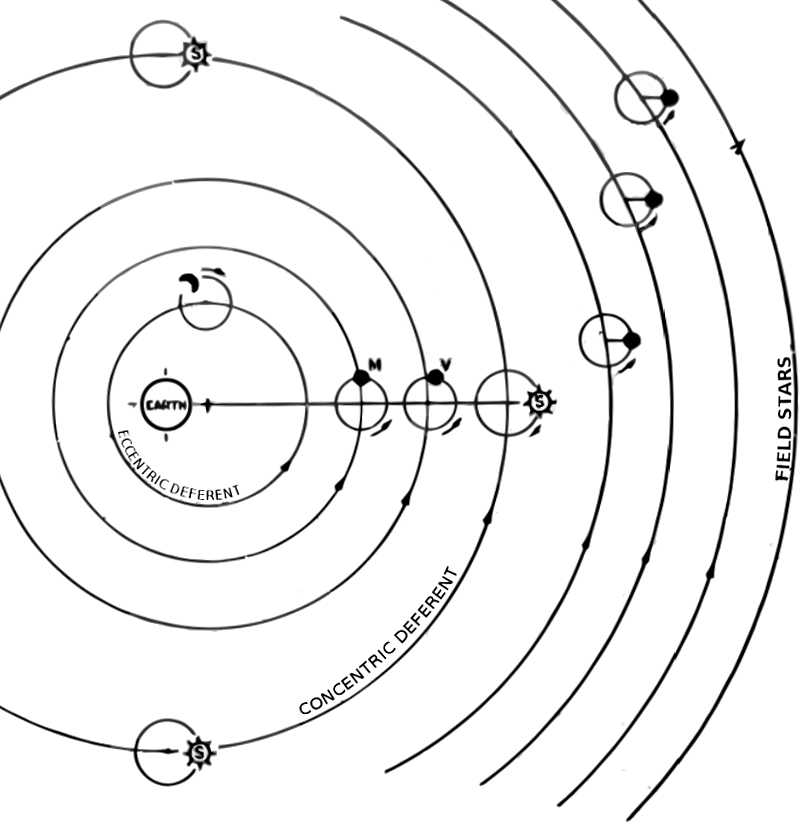
\includegraphics[width=0.9\linewidth]{Figures/0_PtolemaicModel_2.png}
        \caption{Ptolemy geocentric system}
        \label{Fig:0_ptolemaicsystem}
    \end{subfigure}
    ~~
    \begin{subfigure}[b]{0.48\textwidth}
    	\centering
    	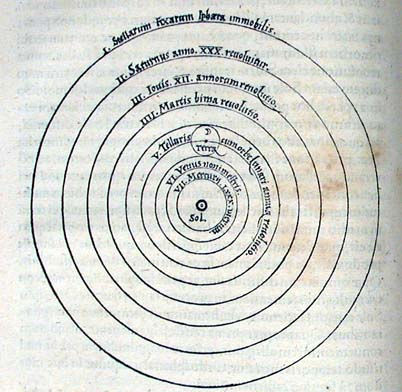
\includegraphics[width=\linewidth]{Figures/0_CopernicusModel.jpg}
        \caption{Copernic heliocentric system}
        \label{Fig:0_copernicsystem}
    \end{subfigure}
\caption{(a): depiction of the Ptolemaic geocentric system, the equant is not shown. (b): Copernicus illustration of his own heliocentric system, from \textit{De revolutionibus}.}
\label{Fig:0_heliogeo}
\end{figure}



The astronomical evidence was, at the time, paradoxically against him. The apparent size changes of planets could not be measured yet, as well as stellar parallaxes, contradicting heliocentrism. The idea of a moving Earth implied some effect on falling bodies (known today as Coriolis effect) which were also not measurable at the time. Building on this apparent counter-evidence and on the work of indian astronomer Nilakantha Somayaji, Tycho Brahe, the most renowned astronomer of his time, proposed an alternative model known as the Tychonic system in the late 16th century \citep{ramasubramanian1998}. Brahe maintained the Earth as the center of the universe, circled by the sun, itself orbited by all other planets. The system was very efficient and was quickly adopted by the Church and considered in compliance with the Holy Scriptures.

However, the seed of heliocentrism was planted in European scientific minds. The idea exalted the impetuous and visionary Giordano Bruno, who pushed the decentralization of Earth to the extreme, claiming stars were other suns, harbouring other planets, which themselves could sustain intelligent life. For this, his rejection of catholic dogma and his vehement refusal of retraction, Bruno was burned at the stake on the Campo de Fiori in 1600. Bruno, the fiery dialectist, despised geometry and believed the mind alone could unravel any mystery. 

Johanes Kepler believed in geometry, in consistency and in observations. Ardent supporter of copernicism, he convinced Tycho Brahe to grant him access to his astronomical data, unsurpassed at the time. Focusing on the motion of Mars, Kepler, through trial and error, found out the planet was moving around the Sun following an ellipse. He formulated his first two laws of planetary motions. Further exploration led him to the third law. The three laws of Kepler of planetary motion were formulated, initiating the mathematisation of astronomy. They are:

\begin{quote}
Law I : All planets orbits are ellipses, with the Sun at one focus.
\end{quote}

\begin{quote}
Law II: The line connecting a planet and the Sun sweeps out equal areas in equal amounts of times as the planet follow its orbit.
\end{quote}
 
 \begin{quote}
 Law III: The squared orbital period of a planet is proportional to the cubed semi-major axis of its orbit.
 \end{quote}


\subsection*{The Starry Messenger}


The father of modern astronomy, and precursor of modern science, Galileo Galilei was born in Pisa in 1564. For the first part of his scientific career, Galileo got famous for his lectures on mechanics and motion. Building on Buridan and Oresme's ideas, he expressed the mathematical form of free fall motion $ d = \frac{gt^2}{2}$. Galileo also formulated what was essentially the future first law of motion from Newton.

In 1609, his passion for scientific instruments led Galileo to build his own "dutch perspective glass", or telescope, a pioneering optical device from the Netherlands. Once pointed at the sky, the device triggered an avalanche of observations which would forever bury the aristotelitian view of perfect and unchanged heavens. Moving Jupiter satellites, Moon craters and mountains, millions of stars in the Milky Way, these were consigned into \textit{Sidereus Nuncius} (Starry messenger), the first scientific publication of astronomical observations \citep{galileo1610}.

Strong advocate of copernicism, but lacking proper evidence, Galileo caused a large controversy with his 
\textit{Dialogue Concerning the Two Chief World Systems} published in 1632, a pamphlet against the ptolemaic system, presenting (arguably unintentionally) one of its advocates as a simpleton. Despite his friendship with the pope, he had to retract his work and reject copernicism. Galileo spent the rest of his life under house arrest. Observational evidence at the time was still on the side of geocentrism. However, the extent of the backslash against Galileo showed the agitation of a Church having absorbed Ptolemy and Aristotle principles into its doctrine, in a time seeing the debate shift from theology to physics and observations.

\begin{figure}
\center
    \centering
    \begin{subfigure}[b]{0.3\textwidth}
    	\centering
    	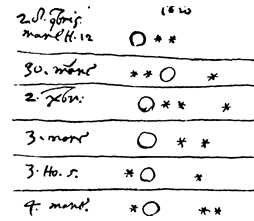
\includegraphics[width=\linewidth]{Figures/0_galileodrawings_1.png}
        \caption{Jupiter satellites}
        \label{Fig:0_galileo_1}
    \end{subfigure}
    ~~
    \begin{subfigure}[b]{0.3\textwidth}
    	\centering
    	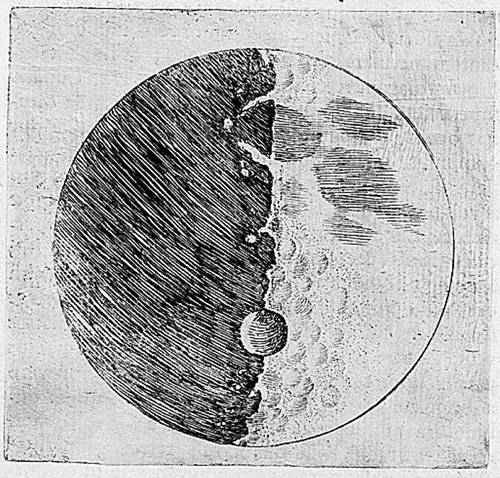
\includegraphics[width=0.9\linewidth]{Figures/0_galileodrawings_2.jpg}
        \caption{Half-moon}
        \label{Fig:0_galileo_2}
    \end{subfigure}
        ~~
    \begin{subfigure}[b]{0.3\textwidth}
    	\centering
    	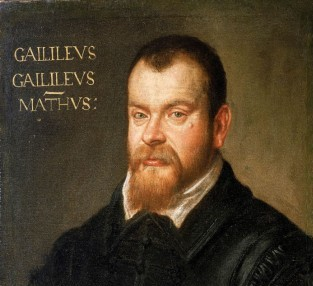
\includegraphics[width=\linewidth]{Figures/0_young_galileo.jpg}
        \caption{Galileo (1605)}
        \label{Fig:0_galileo_3}
    \end{subfigure}
\caption{(a) and (b): drawings by the hand of Galileo of his astronomical observations.}
\label{Fig:0_galileo}
\end{figure}


The relativity of motion is often attributed to Galileo, as he includes it in his controversial pamphlet, stating that a traveller inside a ship sailing smoothly would not be able to tell he's moving. Thus, people could be standing on a moving Earth without feeling it. However, this thought experiment was nothing new at the time and had been a recurring theme of mechanical philosophy since Buridan. Oresme, Copernicus and Bruno had been building on the idea, expanding and improving it, developing over the centuries an implicit understanding of inertia, until Bruno actually gives it a name: \textit{virt\`u}. Galileo may have met Bruno himself, and had surely been influenced by his writings \citep{DeAngelis2015}. Galileo's formulation was clearer, and part of a larger understanding of motion, introducing the concept of reference frame. After Copernicus decentralized the Earth, Galileo decentralized human subjectivity itself, setting the scene for the revolution to come. 

\subsection*{On the shoulders of giants}

Isaac Newton is without a doubt the father of modern mathematical science. Admitted in Cambridge in 1661, Newton supplemented the -still- official aristotelitian teaching with more modern authors: Copernicus, Galileo, Kepler, and most of all, Descartes. The french philosopher had a profound impact on the young student, rooting his love for mathematics and deductive reasoning. However, while Descartes showed disdain for experimentation, Newton was an acute observer of the natural world. 

In 1666, while in is mother's farm, having been forced out of Cambridge by the Plague, Newton began his reflection on the motion of celestial bodies. He derived from Kepler's law that the Sun had to exert an inverse squared distance attraction on the planets. Extending the concept to the Earth, moon, and a famous apple, Newton found a way to verify his hypothesis, using data from Galileo mechanical studies on the strength of Earth attraction. The wrong estimate of Earth radius he used at the time introduced a discrepancy which put the young man off his \textit{gravitas} studies for 18 years.


\begin{figure}
\center
    \centering
    \begin{subfigure}[b]{0.35\textwidth}
    	\centering
    	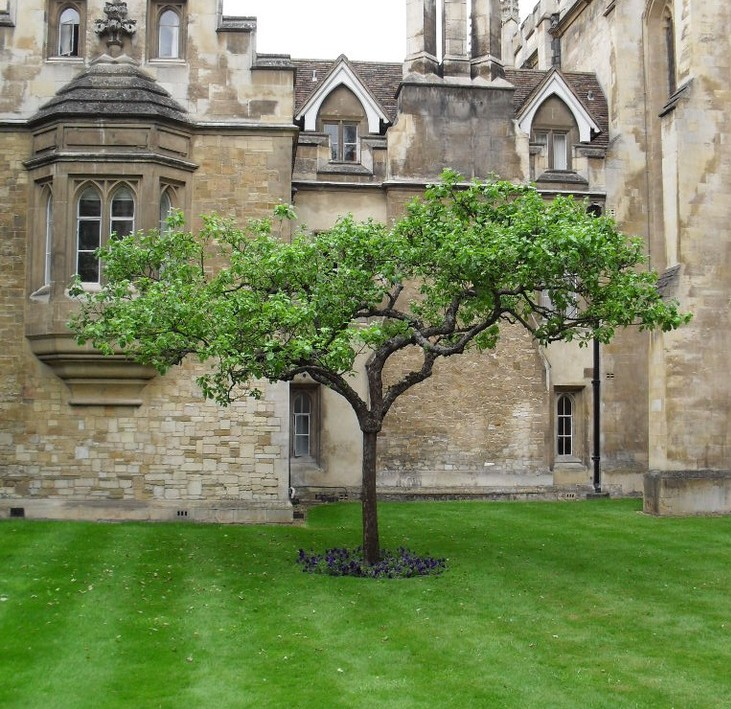
\includegraphics[width=\linewidth]{Figures/0_newtontree.jpg}
        \caption{"Not quite Newton's tree"}
        \label{Fig:0_newton_1}
    \end{subfigure}
    \begin{subfigure}[b]{0.36\textwidth}
    	\centering
    	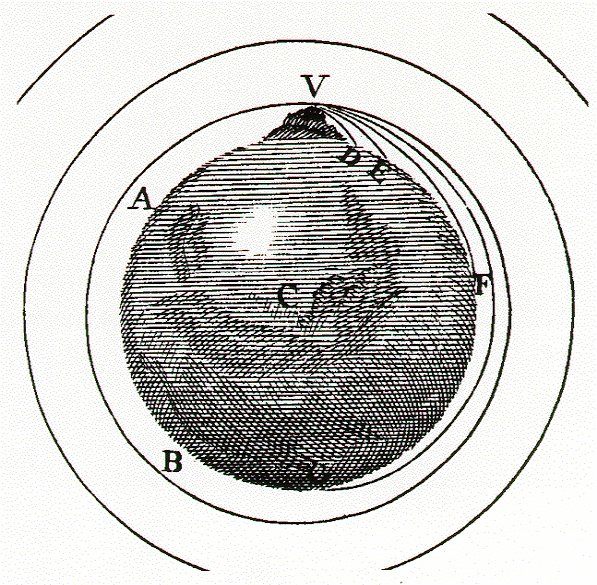
\includegraphics[width=0.9\linewidth]{Figures/0_newtoncannon.jpg}
        \caption{Drawing from the \textit{Principia}}
        \label{Fig:0_newton_2}
    \end{subfigure}
        \\
    \begin{subfigure}[b]{0.36\textwidth}
    	\centering
    	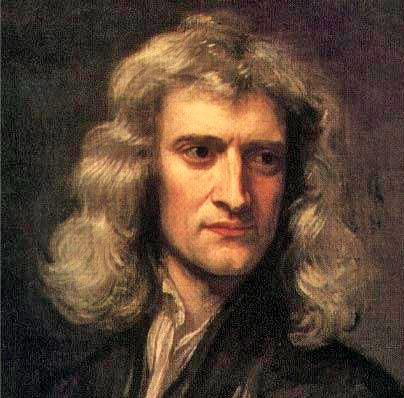
\includegraphics[width=\linewidth]{Figures/0_newtonportrait.jpg}
        \caption{Isaac Newton (1689)}
        \label{Fig:0_newton_3}
    \end{subfigure}
        \begin{subfigure}[b]{0.35\textwidth}
    	\centering
    	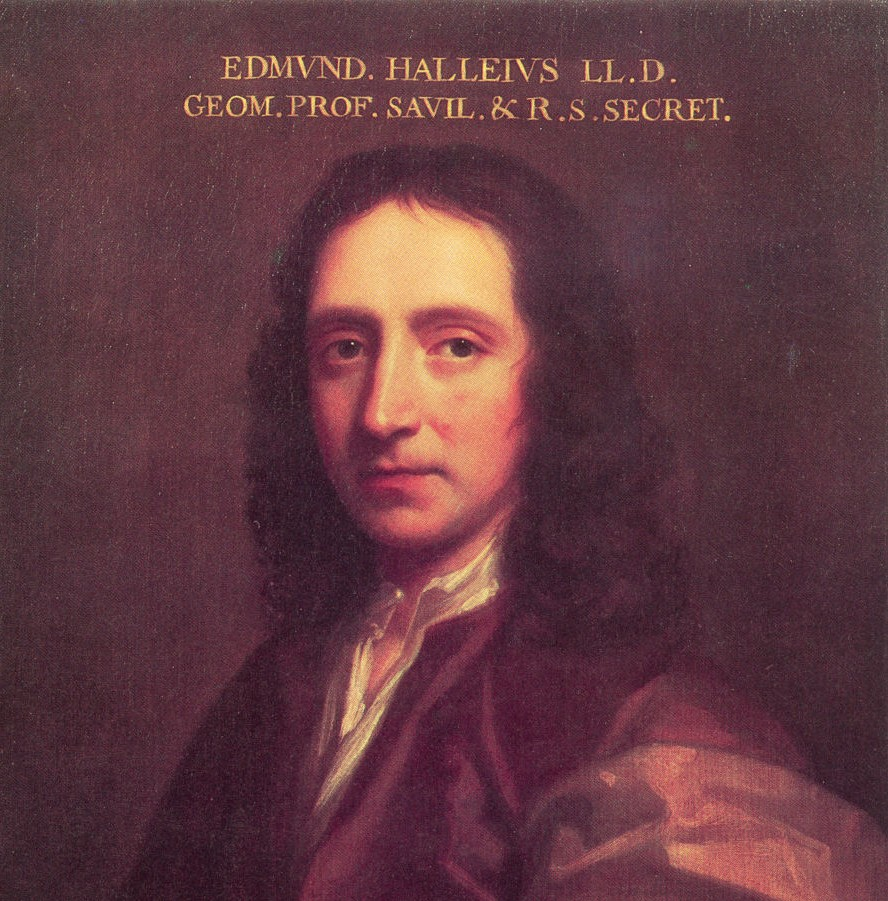
\includegraphics[width=\linewidth]{Figures/0_newtonhalley.jpg}
        \caption{Edmund Halley (1686)}
        \label{Fig:0_newton_4}
    \end{subfigure}
\caption{(a) a supposedly descendant from Newton's apple tree in Cambdrige. The drawing in (b) illustrates the common mechanics of cannonballs and satellites.}
\label{Fig:0_newton}
\end{figure}


Edmund Halley, astronomer and friend of Newton, having heard of Newton inverse squared law, urged him in 1684 to communicate his work the Royal Society. With a new accurate measure of Earth radius and confronted to a concurrent claim to his law from Robert Hooke \citep{Kramer1982}, Newton capitulated to Halley's eager enthusiasm and communicated his work in the famous \textit{Philosophiæ Naturalis Principia Mathematica} \citep{Newton1687}. Published at Halley's own expense, the Principia shook all of Europe. Newton had invented Calculus (in parallel of Leibniz) and applied it to derive the universal law of Gravitation.

\begin{equation}
F = G \frac{m_1.m_2}{r^2}
\end{equation}


Where:
\begin{itemize}
 \setlength\itemsep{-0.5em}
  \item[$F$] Gravitational attraction between object 1 and object 2
\item[$G$] Gravitational constant, $6.67408.10^{-11} m^3 kg^{-1} s^{-2}$ \citep{Pavese2015}
\item[$m_i$] Masses of object 1 and 2
\item[$r$] Distance between object 1 and 2
\end{itemize}

Though Newton was part of continuous line of geniuses and innovative minds building from each others, as he puts it "If I have seen further it is by standing on the shoulders of giants" \citep{Maury1992}, his input was truly revolutionary. He made large advances in optics and mathematics, and created a consistent mathematical framework to compute motions, essentially founding modern science and sowing the seeds of the industrial revolution. This framework is summed up by Newton's three laws of motion (from recent translation \citealt{Cohen1999}):

\begin{quote}
Law I : Every body persists in its state of being at rest or of moving uniformly straight forward, except insofar as it is compelled to change its state by force impressed.
\end{quote}

\begin{quote}
Law II: The alteration of motion is ever proportional to the motive force impress'd; and is made in the direction of the right line in which that force is impress'd.
\end{quote}
 
 \begin{quote}
 Law III: To every action there is always opposed an equal reaction: or the mutual actions of two bodies upon each other are always equal, and directed to contrary parts.
 \end{quote}

The second law can be mathematically formulated in more modern terms:

\begin{equation}
\sum \bold{F} = \frac{d \bold{p}}{dt}
\end{equation}

Meaning the sum of all forces $\bold{F}$ applied to an object is equal to the time derivative of its momentum $\bold{p} = m.\bold{v}$.



\subsection*{The N=3 body problem}

As the Enlightenment brought a scientific revolution in many fields, I will now limit the discussion to the development of celestial mechanics, while acknowledging input from other fields.

While the two-body problem had been solved by Newton and expanded by Bernoulli in 1710 \citep{Barrow1997}, in the 18th century the three-body problem remained the object of much investigation and development. A general solution for the Earth-Moon-Sun system would have had applications on nautical astronomy and trans-continental navigation. Extended analytical work by d'Alembert, Clairaut, Euler and Lagrange led to the development of early families of approximate solutions or exact solutions to special cases.

From 1773 to 1793, Joseph-Louis Lagrange, helped by his invention of Lagrangian mechanics, would make a lot of advances on the three-body problem. He introduced the concept of potential and discovered libration points (later known as Lagrange points). In the same time, Pierre-Simon de Laplace proved the stability of the solar system using a newly developed perturbation theory. The solar system dynamics were being unraveled, with finely tuned perturbation computation, but the general three-body problem remained unsolved.

In 1888, Henri Poincar\'e, a renowned mathematician, submitted an entry to a contest sponsored by the King of Sweden Oskar II. The goal was to determine a usable solution to the N-body problem, for any given N. While Poincar\'e does not submit a complete solution, he wins the contest by presenting an in-depth exploration of the phase-space of the restricted three-body problem, which would later give rise to Chaos theory, see \cite{Yoccoz2010}. Poincar\'e managed to prove that the three-body problem had no  solution involving simple functions.

Contrary to popular belief, the three-body problem \textit{has} a solution, it was derived by Karl F. Sundman in 1912 \citep{Sundman1912}. However, any attempt to obtain accurate trajectory predictions would face an enormous convergence time, making the solution unusable in practice \citep{Beloriszky1930}.

It is interesting to note that Elis Str\"omgren performed by-hand calculation of a three-body system, see \cite{Aarseth2003,Stromgren1909}, prefiguring the advent of numerical orbit computation.

\subsection*{The N$>$3 body problem}

\begin{quote}
"The Sun attracts Jupiter and the other planets, Jupiter attracts its satellites and similarly the satellites act on one another."
\end{quote}



\begin{figure}
\center
    \centering
    \begin{subfigure}[b]{0.45\textwidth}
    	\centering
    	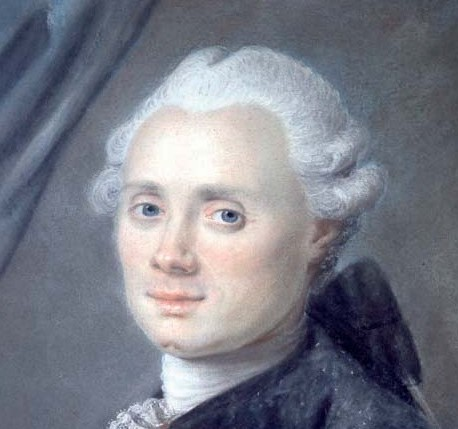
\includegraphics[width=0.84\linewidth]{Figures/0_messier.jpg}
        \caption{Charles Messier (1770)}
        \label{Fig:0_messier}
    \end{subfigure}
    \begin{subfigure}[b]{0.45\textwidth}
    	\centering
    	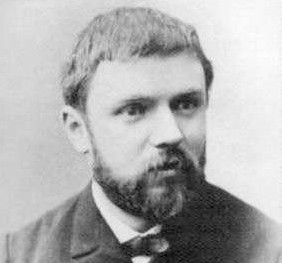
\includegraphics[width=0.84\linewidth]{Figures/0_poincare.jpg}
        \caption{Henri Poincar\'e (1887)}
        \label{Fig:0_poincare}
    \end{subfigure}
\caption{The observer and the theorist, a century apart.}
\label{Fig:0_messierpoincare}
\end{figure}

By this sentence from the \textit{Principia}, Newton formulates the N-body gravitational problem, an arbitrary number of massive bodies all interacting gravitationally, for the solar system. The "N$>$3-body" problem didn't receive a lot of attention at first, as the unruly three-body problem was on everyone's mind, and a higher-N problem seemed abstract, the solar system example being appropriately dealt in approximations.

In 1764, Charles Messier resolved individual stars in Messier 4, a globular cluster, hundreds of thousands of stars grouped together. Many new clusters were to be found afterwards, extending the catalog of real-life N-body systems. However, nothing was known of their kinematics, the stars were, in a sense, suspended motionless in the sky. This was the case until the advent of Doppler spectroscopy, which allowed astronomer to measure stars velocities \citep{Doppler1842}. Stellar dynamics had begun.

The N$>$3-body problem was still inaccessible, so scientists like James Jeans and Arthur Eddington decided to take the problem from the other hand, and took advantage of the large number of stars. Inspired by \cite{Poincare1906}, both astronomers applied the statistical theory of gas to stellar systems, founding the field of stellar dynamics \citep{Jeans1916,Eddington1916}.

An interesting experiment was conducted by \cite{Holmberg1941} to understand the collision of two stellar systems (galaxies). With too few points to warrant a statistical approach, and before the rise of numerical integration, Holmberg modelled two galaxies with dozens of lightbulbs and photocells, measuring the attractive force with the amount of light received in each direction, taking advantage of the inverse squared fall of luminosity with distance, akin to gravity.

\subsection*{The numerical age}

The first numerical N-body computations were performed by Sebastian Von Hoerner in 1959 when visiting the University of T\"ubingen, on a Siemens 2002, a cutting edge calculator at the time (Fig~\ref{Fig:0_siemens}). The very first had N=4. Then, Von Hoerner, back in Heidelberg, worked his way up to 16 stars, then 25, programming and debugging on punch cards. This story was told by Von Hoerner himself in \cite{VonHoerner2001}. He very quickly realized the importance of binary stars and their impact on computations. He was also able to confirm some theoretical prediction on cluster dynamics, and found a cuspy radial density profile\citep{VonHoerner1960,VonHoerner1963}.

There was two ways to increase the number of stars in simulations: buy a better computer or improve the algorithm. Sverre Johannes Aarseth got invested in the second path, which would take over his scientific life. Aarseth pioneered the use of individual time-step, changing the rate of particle positions update, gravitationnal softening (allowing convergence for close approaches), and polynomial predictions for force calculations \citep{Aarseth1964}. As power and optimization grew, investigations expanded, such as the interaction star-gas \citep{VanAlbada1968a} and binary formation \citep{VanAlbada1968b}.

The 1970s brought two new important optimisation methods: KS regularization of close pairs \citep{Aarseth1972} or 3-body systems \citep{Aarseth1974b} and Ahmad-Cohen neighbour scheme \citep{AhmadCohen1973}. The number of stars in simulations kept growing, reaching 1000 with \cite{Terlevich1980} and materializing into the \textit{NBODY5} integrator. At this point various methods departing from a pure collisional calculation began to emerge, such as the simplified distant interaction with the \cite{BarnesHut1986} tree algorithm.


\begin{figure}
\center
    \centering
    \begin{subfigure}[b]{0.45\textwidth}
    	\centering
    	\includegraphics[width=0.98\linewidth]{Figures/0_siemens2002.jpg}
        \caption{Siemens 2002}
        \label{Fig:0_siemens}
    \end{subfigure}
    \begin{subfigure}[b]{0.45\textwidth}
    	\centering
    	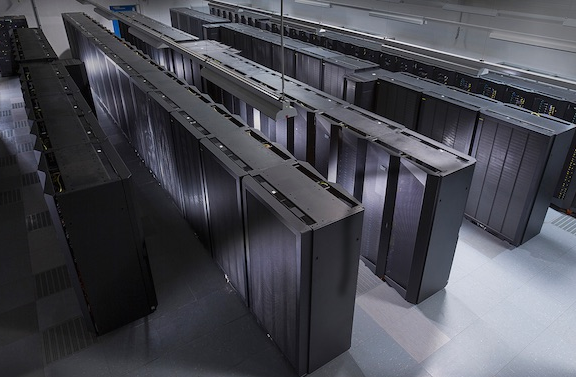
\includegraphics[width=\linewidth]{Figures/0_hydra.png}
        \caption{Hydra supercomputer}
        \label{Fig:0_hydra}
    \end{subfigure}
\caption{The Siemens 2002, seen here on (a) at the computer museum in Kiel, could perform 2000 operations a second. The Hydra cluster, on (b), at the Max Planck Computing \& Data Facility in Garching is made of 83,000 cores and 676 GPUs for a total of $10^{15}$ operations per seconds, a billion millions. }
\label{Fig:0_computers}
\end{figure}

To go beyond the regular improvement of computing power with time, a group of japanese researchers, among whom Junichiro Makino, designed and built special purpose hardware for many-body problems: GRAPE \citep{Ebisuzaki1990,Ito1991}. These cards vastly improved the speed of N-body simulations and were a milestone on the road to the parallelization of computing. With the force calculation directly implemented in the hardware, GRAPE dominated the field for 15 years.

The latest technological leap in N-body simulations came from graphic cards, see \cite{Bedorf2012} for a more detailed historical perspective. Graphical Processing Units, or GPU, were originally designed for computer games visual rendering, applying the same transformations to a lot of pixels at the same time. These made them very efficient parallel computing machines for physics. Interest in GPU computing started to grew in the 2000s \citep{Nyland2004,Elsen2006,SPZ2007} until the advent of usable GPU programming languages, like CUDA, in the late 2000s. At this point GPU were more efficient than GRAPE hardware for force calculation. Keigo Nitadori and Sverre Aarseth developped a GPU-accelerated version of NBODY6 in 2012 \citep{Nitadori2012}. A new iteration of the NBODY family, NBODY7, was also developed to include post-newtonian effects from General Relativity \citep{Aarseth2012}.

\begin{figure}
\label{Fig:N_increase}
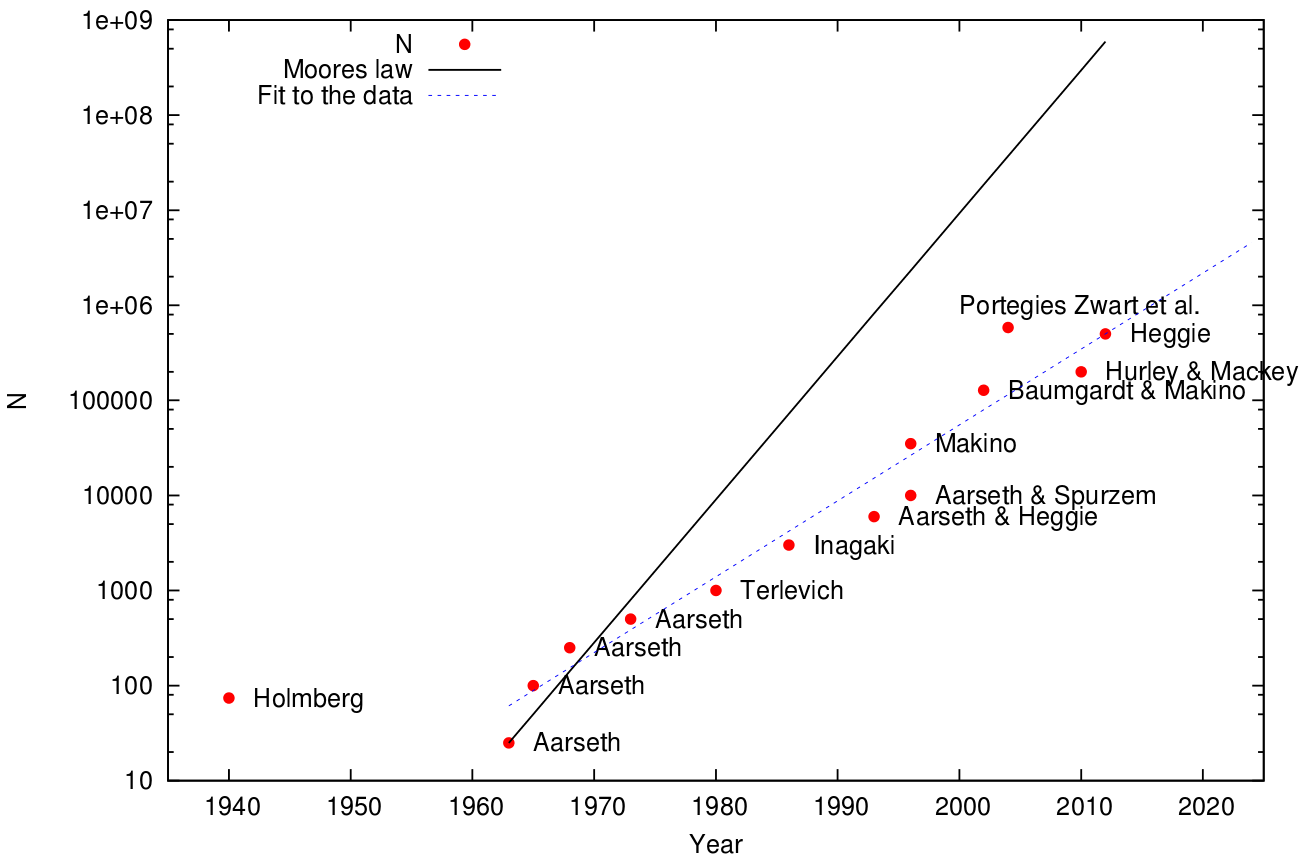
\includegraphics[width=0.9\linewidth]{Figures/0_N_increase.png}
\caption{The evolution of the number of particles in N-body simulations. Solid line shows the Moore law. The figure was taken from \protect\cite{Bedorf2012}. }
\end{figure}


This year, 330 years after the publication of the \textit{Principia}, \cite{Wang2016} performed several collisional nbody simulations of one million stars with a modified version of NBODY6 running on GPUs, on the Hydra supercomputer (Fig~\ref{Fig:0_hydra}). Computers have made it possible for humans to study systems of incredible scales in space and time, only using the universal law of gravitation. N-body numerical integrators are the culmination of centuries of scientific development on the motion of massive bodies.